

\begin{table*}
    \centering
    \large
    \begin{tabular}{l cc   cc  cc}
        \mr{2}{Métrica}          &\mc{2}{Sin Contexto}& \mc{2}{Tweet}          &  \mc{2}{Tweet + Cuerpo}    \\
                                    & $\neg$FT&  FT    & $\neg$FT&    FT  & $\neg$ FT&    FT \\
        \hline
                        Accuracy  & 0.889   &  0.899 & 0.902 &\textbf{0.910} & 0.904 &    0.905 \\
                        Precision & 0.678   &  0.718 & 0.731 &\textbf{0.748} & 0.739 &    0.728 \\
                        Recall    & 0.568   &  0.602 & 0.601 &\textbf{0.653} & 0.611 &    0.641 \\
                        F1        & 0.618   &  0.655 & 0.660 &\textbf{0.697} & 0.669 &    0.681 \\
                        Macro  F1 & 0.776   &  0.798 & 0.801 &\textbf{0.822} & 0.806 &    0.813 \\
        \bottomrule
    \end{tabular}


    \caption{Resultados de los experimentos de clasificación para la tarea \emph{binaria} de detección de discurso de odio. Cada modelo es un BERT con 3 posibles entradas: sólo el comentario (\emph{Sin contexto}), el tweet de la noticia a la cual responde el comentario (\emph{Tweet}), y el tweet más el cuerpo de la noticia (\emph{Tweet + Cuerpo}). Para cada una de estas posibilidades usamos dos versiones: una sobre BETO ($\neg$FT) y otra sobre BETO ajustado al dominio (FT)}
    \label{tab:task_a_results}
\end{table*}


La tabla \ref{tab:task_a_results} contiene los resultados de la tarea de clasificación binaria, medidos por accuracy, precision, recall, F1 de la clase positiva y Macro F1 entre las dos clases, expresados como las medias de 10 corridas independientes de los experimentos. Las seis columnas corresponden a la combinación de los 3 posibles modelos dependiendo del contexto utilizado y de acuerdo a si ajustamos al dominio o no. Podemos observar que, en todos los casos, la adaptación de dominio (las columnas marcadas con FT) obtienen mejor performance que los modelos que no están adaptados ($\neg$FT), resultando en los casos sin contexto y con contexto de tweet en una mejora de alrededor de 4 puntos de F1. Entre los modelos sin ajustar a dominio, el modelo que consume el contexto completo (tweet + cuerpo de la noticia) obtiene el mejor desempeño; sin embargo, el contexto simple mejora esta performance cuando es adaptado. Viendo sólo las columnas adaptadas a dominio ($FT$), la mejora contra el modelo que no consume contexto es de 4.2 puntos de F1. El modelo con el contexto completo, si bien mejora la performance general contra no tener contexto, pierde precisión al ser adaptado al dominio.


\begin{table*}
    \centering
    \Large
    \begin{tabular}{r ll   ll  ll}
        Métrica        &\mc{2}{Sin Contexto}& \mc{2}{Tweet}          &  \mc{2}{Tweet + Cuerpo}    \\
                       & $\neg$FT&    FT    & $\neg$FT   &    FT     & $\neg$ FT&    FT     \\
        \hline
        Calls F1       & 0.646 &    0.651   & 0.638 &\textbf{0.685}  & 0.653 &    0.680    \\
        Women F1       & 0.373 &    0.389   & 0.411 &\textbf{0.421}  & 0.381 &\textbf{0.421} \\
        Lgbti F1       & 0.351 &    0.366   & 0.451 &\textbf{0.482}  & 0.427 &    0.445    \\
        Racism F1      & 0.635 &    0.653   & 0.688 &\textbf{0.720}  & 0.691 &    0.711    \\
        Class F1       & 0.401 &    0.433   & 0.491 &\textbf{0.511}  & 0.451 &    0.476    \\
        Politics F1    & 0.555 &    0.611   & 0.579 &0.625           & 0.591 &\textbf{0.648} \\
        Disabled F1    & 0.551 &    0.582   & 0.585 &\textbf{0.609}  & 0.557 &    0.578    \\
        Appearance F1  & 0.726 &    0.742   & 0.741 &\textbf{0.766}  & 0.755 &    0.758    \\
        Criminal F1    & 0.513 &    0.529   & 0.650 &\textbf{0.699}  & 0.654 &    0.668    \\
        \hline
        Macro F1       & 0.528 &    0.551   & 0.582 &\textbf{0.613}  & 0.573 &    0.598    \\
        Macro Precision& 0.558 &    0.630   & 0.642 &\textbf{0.702}  & 0.677 &    0.678    \\
        Macro Recall   & 0.506 &    0.499   & 0.540 &\textbf{0.551}  & 0.504 &    0.541    \\
        % \hline
        % Hate Precision & 0.679 &    0.712   & 0.722 &\textbf{0.760}  & 0.748 &    0.741    \\
        % Hate Recall    & 0.621 &    0.631   & 0.642 &\textbf{0.666}  & 0.621 &    0.658    \\
        % Hate F1        & 0.648 &    0.668   & 0.679 &\textbf{0.710}  & 0.679 &    0.697    \\
        \bottomrule
        \end{tabular}
    \caption{Performance de los modelos para la tarea de detección granular de discurso de odio. Cada modelo es un BERT con 3 posibles entradas: sólo el comentario (\emph{Sin contexto}), el tweet de la noticia a la cual responde el comentario (\emph{Tweet}), y el tweet más el cuerpo de la noticia (\emph{Tweet + Cuerpo}). Para cada una de estas posibilidades usamos dos versiones: una sobre BETO($\neg$FT) y otra sobre BETO ajustado al dominio (FT) de acuerdo a lo descripto en la sección \ref{sec:contextualized_classifiers}}
    \label{tab:task_b_results}
\end{table*}



La tabla \ref{tab:task_b_results} muestra los resultados de los experimentos de clasificación para la tarea de detección fina, medida en F1 para cada una de las características, y las medidas agrupadas de forma macro precision, recall, y F1. Se muestra en cada caso el resultado de la media de 10 corridas del experimento. Como era esperable, la ganancia de tener contexto disponible es más evidente en esta tarea, con una diferencia de Macro F1 aproximadamente 6 puntos de F1 entre la mejor versión sin contexto y la mejor versión con contexto (0.55 Macro F1 de la versión $FT$ sin contexto vs 0.61 F1 de la versión $FT$ con el contexto del tweet).


\begin{figure*}[t]
    \centering
    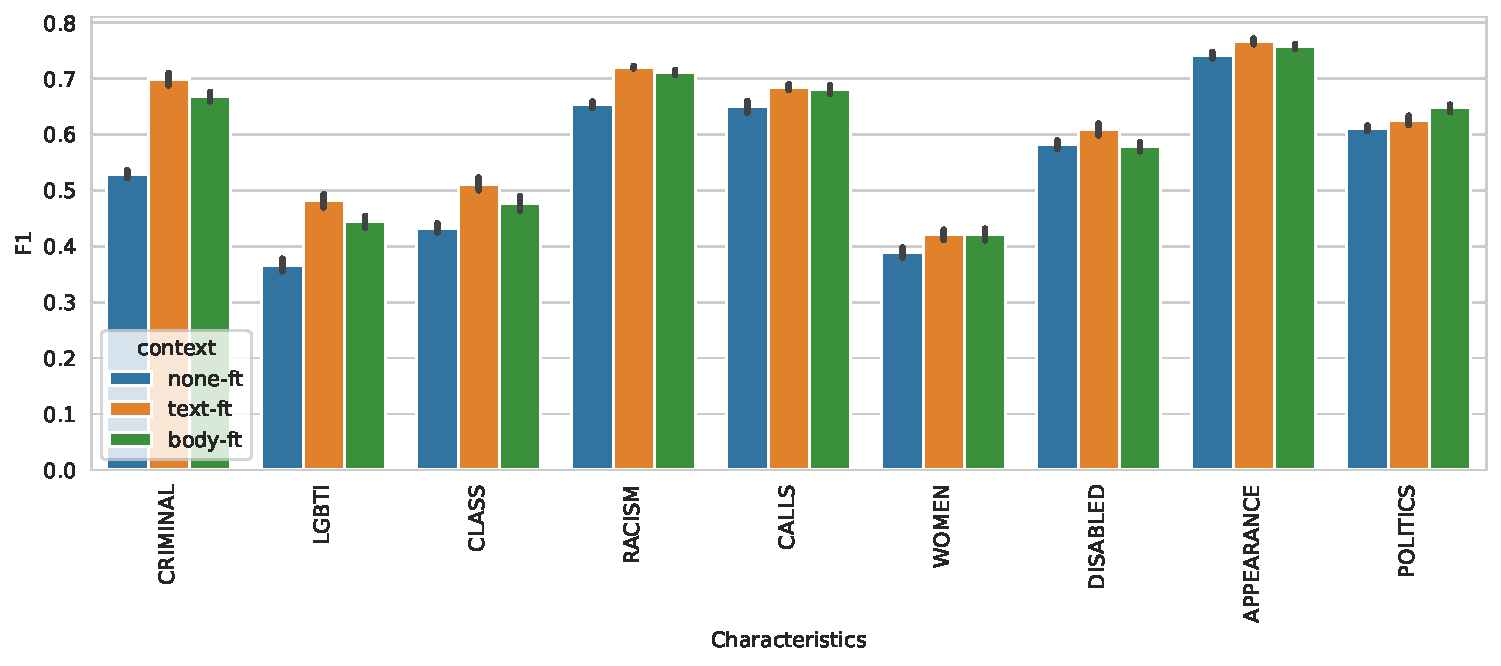
\includegraphics[width=\textwidth]{img/task_b_scores.pdf}
    \caption{Métrica F1 para cada característica de la tarea Task B. Las características están ordenadas de mayor a menor de acuerdo a la diferencia de performance entre el modelo sin contexto y el modelo contextualizado. }
    \label{fig:barplot_task_b_results}
\end{figure*}

La figura \ref{fig:barplot_task_b_results} muestra los resultados de las F1 por característica, esta vez ordenados de mayor a menor según el gap entre la performance contextualizada vs la no contextualizada, junto a sus intervalos de confianza 95\%, usando como modelos las versiones ajustadas al dominio. Todas las características obtienen una mejora estadísticamente significativa al correr un test Mann-Whitney U ($p \leq 0.005$, p valores ajustados por Benjamini-Hochberg \cite{benjamini1995controlling}). Las diferencias más sustanciales se dan en el caso de CRIMINAL ($+0.17$ F1 de diferencia), LGBTI ($+0.12$), CLASE ($+0.08$), y RACISMO (casi $+0.07$). Del otro lado, las características con menos mejora son APARIENCIA y POLITICA, algo esperable dado que el fenómeno tiene características poco dependientes del contexto (ver Apéndice \ref{app:manual_criterios_anotacion} para ejemplos). Finalmente, y como resumen de estas tablas, se observa que los modelos con contexto simple (que consumen sólo el tweet) son los que mejor performance tienen, en general y para cada característica, con la excepción de POLITICA.


\begin{figure}[ht]
    \centering
    \small
    \begin{subfigure}[b]{\textwidth}
        \centering
        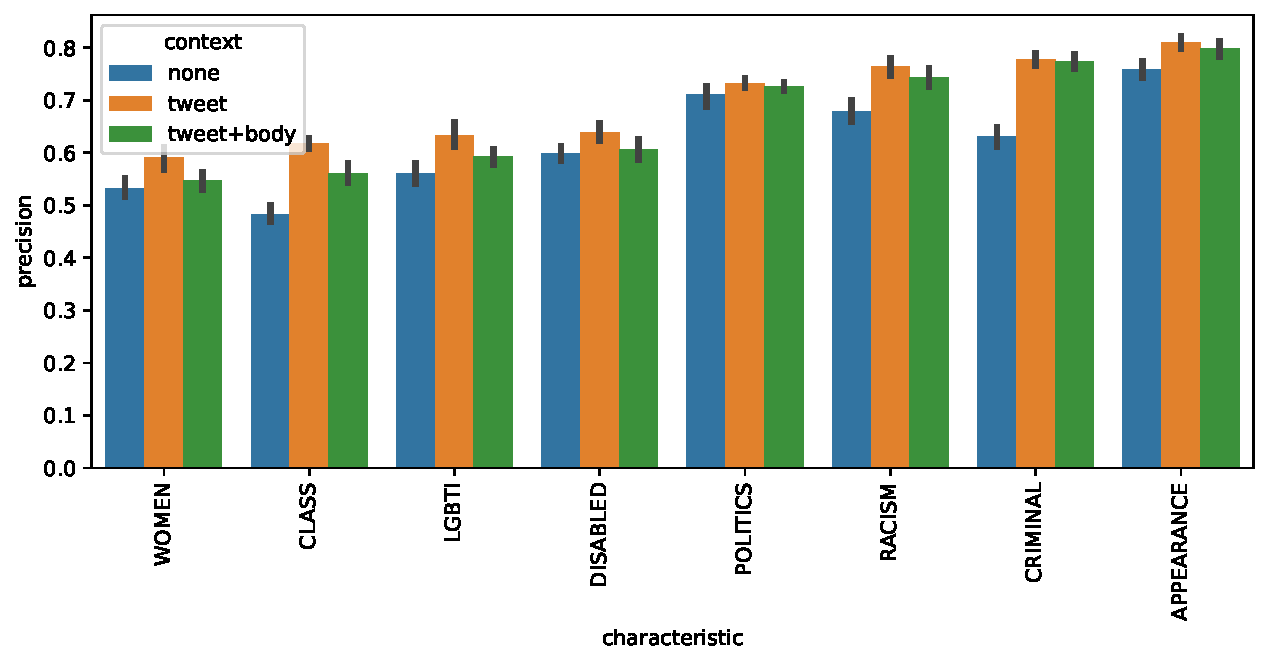
\includegraphics[width=0.85\textwidth]{img/context_classification/precision_barplot.pdf}
        \caption{Precisión}
    \end{subfigure}
    \begin{subfigure}[b]{\textwidth}
        \centering
        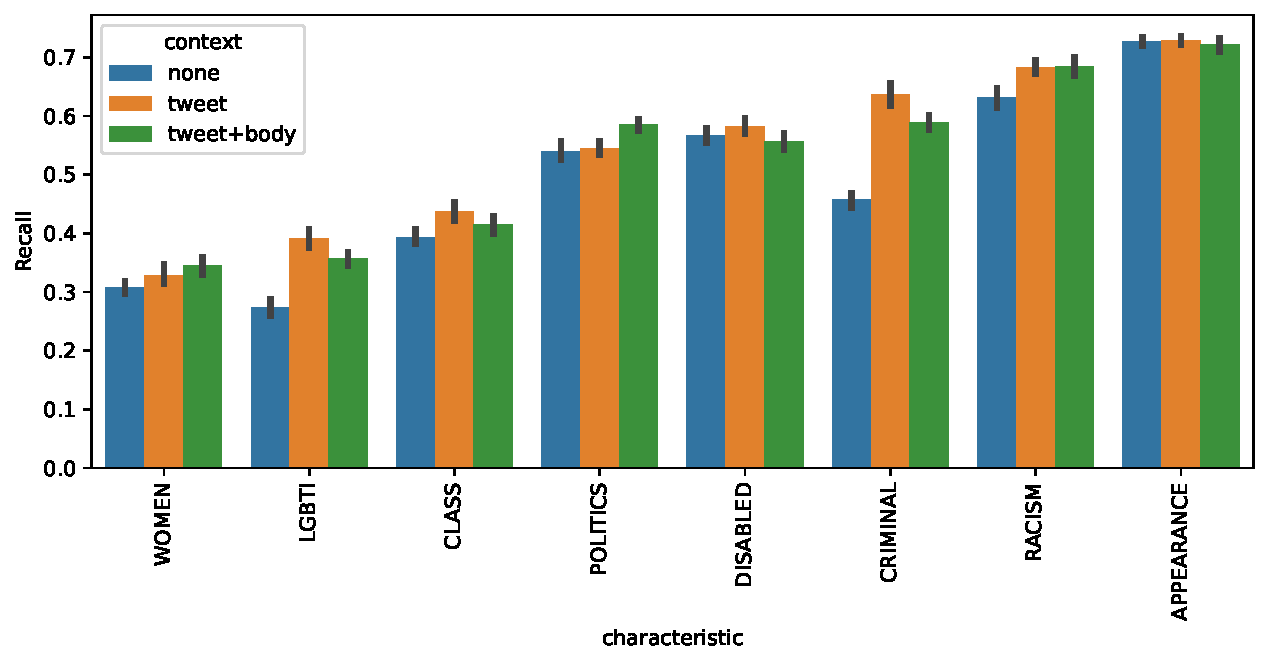
\includegraphics[width=0.85\textwidth]{img/context_classification/exact_recall_barplot.pdf}
        \caption{Recall exacto}
        \label{subfig:exact_recall}
    \end{subfigure}
    \begin{subfigure}[b]{\textwidth}
        \centering
        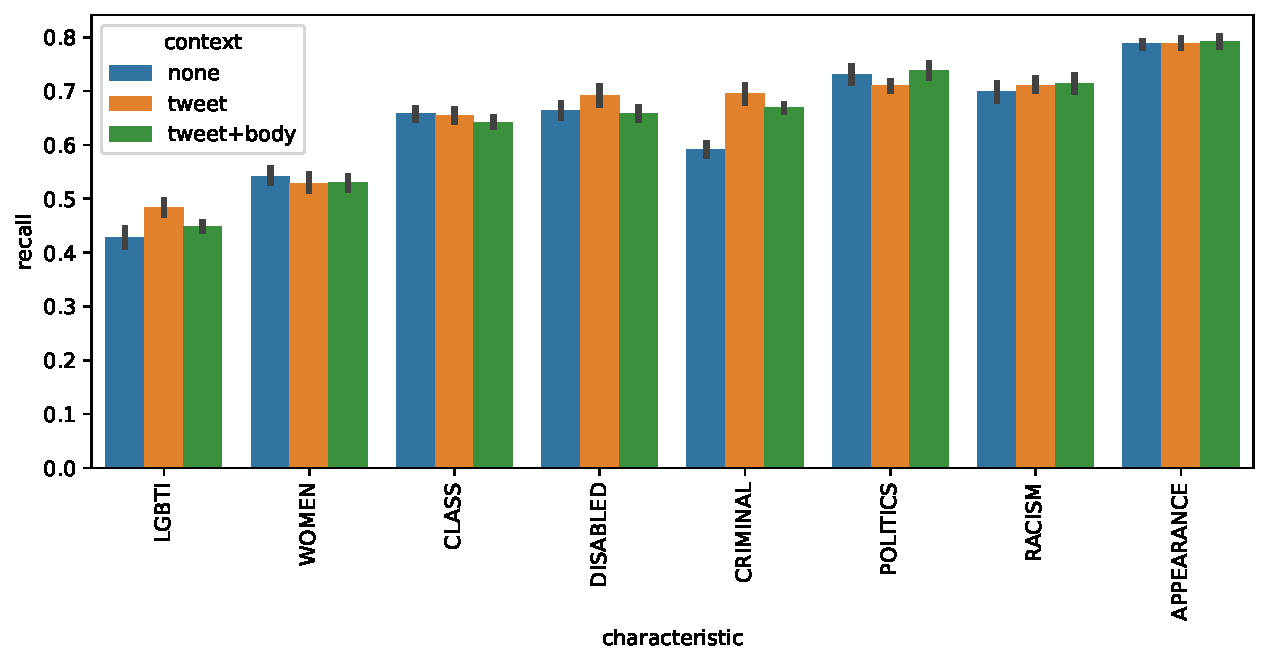
\includegraphics[width=0.85\textwidth]{img/context_classification/hate_recall_barplot.pdf}
        \caption{Recall por categoría}
        \label{subfig:total_recall}
    \end{subfigure}
    \caption{Precision y Recall para cada característica de la tarea Task B. Las diferentes barras marcan el tipo de entrada que recibe el clasificador basado en \beto{}. Recall exacto (Figura \ref{subfig:exact_recall}) cuenta el recall sobre la salida de cada categoría (es decir, sólo cuenta como recuperado un tweet marcado como MUJER si la salida del clasificador es MUJER). Recall total cuenta como recuperado un tweet si al menos alguna característica del clasificador lo marca como discurso de odio.}
    \label{fig:precision_recall}
\end{figure}

La tabla \ref{fig:precision_recall} muestra la precisión y recall/sensibilidad de los clasificadores de la tarea granular. La sensibilidad es analizada de dos maneras: exacta, donde consideramos recuperado un tweet sólo si el clasificador acierta a la característica analizada (es decir, si la característica es MUJER, tiene que decir MUJER); y total, donde consideramos un tweet recuperado si alguna característica se enciende, independientemente si es la adecuada. Podemos ver que la categoría MUJER pasa de ser la de menor sensibilidad a dejar a la categoría LGBTI como la que tiene menor cantidad de recuperados. Análogamente la categoría CLASE obtiene una mejora sustancial en su sensibilidad, otra que es esperable que tenga cierta mezcla con otras características como RACISMO y posiblemente CRIMINAL.

\begin{table*}
    \centering
    \footnotesize
    \begin{tabular}{l |cc  | cc | cc}
        Métrica        &\mc{2}{Sin Contexto}& \mc{2}{Tweet}          &  \mc{2}{Tweet + Cuerpo}    \\
                       & Plano &    Granular    & Plano   &    Granular     & Plano &   Granular     \\
        \hline
        precision &  $0.718 \pm 0.016$ &  $0.711 \pm 0.022$ &  $0.748 \pm 0.019$& $0.759 \pm 0.013$ & $0.728 \pm 0.024$ & $0.740 \pm 0.015$ \\
        recall    &  $0.602 \pm 0.014$ &  $0.636 \pm 0.015$ &  $0.653 \pm 0.014$& $0.667 \pm 0.013$ & $0.641 \pm 0.023$ & $0.660 \pm 0.015$ \\
        F1        &  $0.655 \pm 0.004$ &  $0.671 \pm 0.003$ &  $0.697 \pm 0.003$& $0.710 \pm 0.006$ & $0.681 \pm 0.006$ & $0.697 \pm 0.004$ \\
        Macro F1  &  $0.798 \pm 0.002$ &  $0.806 \pm 0.002$ &  $0.822 \pm 0.002$& $0.830 \pm 0.003$ & $0.813 \pm 0.003$ & $0.822 \pm 0.002$ \\        \bottomrule
        \end{tabular}
    \caption{Performance de los modelos para la tarea de detección de discurso de odio. Los modelos son BERT ajustados a dominio, consumiendo los 3 tipos de contexto: sin contexto, con contexto de tweet, y con contexto completo (tweet+cuerpo). Comparamos la performance entre los clasificadores que fueron entrenados sobre la tarea \textbf{binaria} y la tarea \textbf{granular}}
    \label{tab:plain_vs_granular_hate_detection}
\end{table*}


Como se mencionó en la sección \ref{sec:tasks}, un clasificador sobre la tarea granular puede convertirse fácilmente en un clasificador para la tarea binaria tomando la disyunción lógica de sus salidas: si al menos una salida es 1, entonces el tweet es discurso de odio. Analizamos así el desempeño en la tarea binaria de aquellos clasificadores entrenados granularmente. La tabla \ref{tab:plain_vs_granular_hate_detection} muestra esta comparativa. Podemos observar que en todos los casos, entrenar el modelo sobre la tarea granular produce mejoras pequeñas pero significativas en la performance de los clasificadores entrenados sobre la tarea binaria.



